\chapter{De la tipare secventiale frecvente la silabisire}
\label{cap:contributii}

În cadrul acestui capitol se prezenta în detaliu metoda propusă, prin care, pornind de tipare secvențiale frecvente, se pot identifica despărțiri în silabe ale cuvintelor.  

\section{Prezentare de ansamblu a soluției}

\begin{figure}[h]
    \centering
    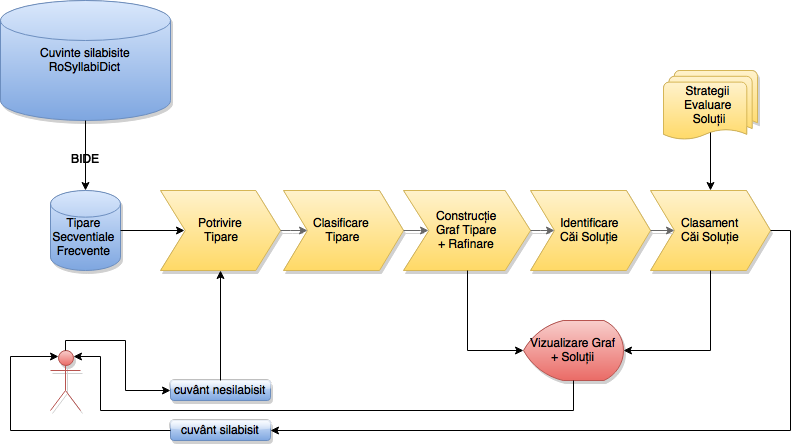
\includegraphics[width=\textwidth]{figures/rosil-flow.png}
    \caption{Diagrama conceptuală a soluției propuse}
    \label{fig:rosil-flow}
\end{figure}

Principalele etape ale metodei sunt următoarele:
\begin{enumerate}
\item Identificarea tiparelor frecvente dintr-un set de cuvinte despărțite în silabe și indexarea acestora.
\item Identificarea tiparelor care prezintă un grad ridicat de potrivire în cadrul cuvântului care se dorește a fi despărțit în silabe
\item Clasificarea acestor tipare în funcție poziția în cuvânt pe care au "potrivit-o" (început, sfârșit, interior).
\item Construirea unui graf cu aceste tipare pe baza potrivirii dintre aceste tipare
\item Eliminarea nodurilor izolate din acest graf
\item Pe baza unor strategii de predicție, se va alege o cale sau mai multe în acest graf, reprezentând soluțiile propuse pentru despărțirea în silabe.
\end{enumerate}

\section{Identificarea tiparelor frecvente}

Pentru a construi setul de tipare frecvente a fost folosită colecția de cuvinte despărțite în silabe în limba română RoSyllabiDict, \cite{bib:BARBU08.495}. Acest set de date conține 525486 de cuvinte despărțite în silabe. 

În vederea analizei setului de date, în cadrul tabelului \ref{table:sdb_counts} se poate observa variația numărului de tipare secvențiale frecvente închise în funcție de valoarea de suport minim.   

\begin{table}[h!]
\centering
\begin{tabular}{|c|c|c|c|c|c|c|c|c|}
\hline
Sup.& Total & Lung. 1 & Lung. 2 & Lung. 3 & Lung. 4 & Lung. 5 & Lung. 6 & Lung. 7\\ 
\hline
\hline
1000 & 648 & 252 & 385 & 11 & 0 & 0 & 0 & 0\\ 
\hline
800 & 890 & 293 & 576 & 21 & 0 & 0 & 0 & 0\\ 
\hline
600 & 1339 & 380 & 903 & 56 & 0 & 0 & 0 & 0\\ 
\hline
400 & 2211 & 523 & 1544 & 143 & 1 & 0 & 0 & 0\\ 
\hline
200 & 4812 & 832 & 3384 & 576 & 20 & 0 & 0 & 0\\ 
\hline
100 & 10461 & 1234 & 6754 & 2309 & 162 & 2 & 0 & 0\\ 
\hline
50 & 22852 & 1824 & 12671 & 7453 & 853 & 47 & 4 & 0\\ 
\hline
20 & 62549 & 2597 & 25731 & 28056 & 5384 & 674 & 90 & 17\\ 
\hline
10 & 129106 & 3271 & 41126 & 63388 & 17812 & 2940 & 454 & 97\\ 
\hline
5 & 256065 & 4146 & 63443 & 123429 & 52271 & 10553 & 1840 & 327\\ 
\hline
2 & 633195 & 5469 & 104254 & 248227 & 186623 & 66915 & 16920 & 3882\\ 
\hline\end{tabular}
\label{table:sdb_counts}
\caption{Numărul de tipare secvențiale frecvente închise pentru setul de date RoSyllabiDict} 
\end{table}

Alegerea unui suport minim cat mai mic asigură prezența a cât mai multor tipare în colecția de tipare folosite ulterior de metodă. Aceasta va creste precizia metodei dar pe de altă parte performanța este influențată de cantitiatea de tipare. 

Cu cât numărul de tipare este mai mare, cautarea de potriviri devine mai lentă, iar pentru a creste performanța, acestea pot fi indexate. În tabelul \ref{table:sdb_patterns} sunt prezentate o serie de tipare frecvente, pentru a le indexa metoda se folosește de o tabela de disperie în care valorile cheilor vor fi reprezentate de silabele concatenate continute de tipare. Un astfel de exemplu se regăseste în cadrul tabelului \ref{table:sdb_index}. 

\begin{table}[h!]
\centering    
\begin{tabular}{|l|l|}    
\hline      
Cheie & Valoare\\
\hline
$a$ 		& $(<a>, 2)$  \\
$libe$ 		& $(<li, be>, 2)$  \\
$programa$ 	& $(<pro, gra, ma>, 2)$  \\
$mare$ 		& $(<ma, re>, 2)$  \\
$mator$ 	& $(<ma, tor>, 2)$  \\
$ti$ 		& $(<ti>, 2)$  \\
$eli$ 		& $(<e, li>, 3)$  \\
$grama$ 	& $(<gra, ma>, 3)$  \\
$sare$ 		& $(<sa, re>, 3)$  \\
$tor$ 		& $(<tor>, 4)$  \\
$li$ 		& $(<li>, 4)$  \\
$e$ 		& $(<e>, 5)$  \\
$ma$ 		& $(<ma>, 5)$  \\
$re$ 		& $(<re>, 6)$  \\
\hline
\end{tabular}
\caption{Exemplu de indexare pentru tipare secvențiale frecvente}
\label{table:sdb_index}               
\end{table}  

Odată având colecția de tipare frecvente indexată, procesul de silabizarea poate fi initial. 
 
\section{Potrivirea tiparelor in vederea silabisirii}

Fie $W$ un cuvânt compus dintr-o secvență de litere, iar $Z_W$ mulțimea tuturor subsecventelor continue ale acestui cuvânt, precum si îndexii de inceput și sfârșit ai acestora.

\begin{ex}
Pentru cuvântul $amator$, tuplele din multimea sunt $Z_{amator}$ sunt ilustrate în cadrul tabelului \ref{table:sdb_substrings}. 
\end{ex}


\begin{table}[b!]
\centering    
\begin{tabular}{|l|l|}    
\hline      
Secventă & Indexi\\
\hline
$a$ 		& $\left[0,1\right), \left[2,3\right)$  \\
$m$ 		& $\left[1,2\right)$  \\
... 		& ...  \\
$amator$ 	& $\left[0,6\right)$  \\

\hline
\end{tabular}
\caption{Mulțimea $Z_{amator}$}
\label{table:sdb_substrings}               
\end{table}  

\begin{defi} Prin \textbf{potrivirea tiparelor} pentru cuvântul $W$, având multimea $Z_W$ asociată, se dorește identificarea tuturor tiparelor frecvente care sunt indexate cu chei care aparțin multimii $Z_W$. Notăm rezultatul acestei operații cu $M_W$. Considerând același cuvânt $amator$, $M_{amator}$ este ilustrată în tabelul \ref{table:sdb_pattern_match}
\end{defi}

\begin{table}[h!]
\centering    
\begin{tabular}{|l|l|}    
\hline      
Tipar frecvent & Indexi potrivire\\
\hline
$(<a>, 2)$			& $\left[0,1\right), \left[2,3\right)$   \\
$(<ma>, 5)$  		& $\left[2,4\right)$\\
$(<ma, tor>, 2)$ 	& $\left[2,6\right)$ \\
$(<tor>, 4)$  		& $\left[4,6\right)$\\
\hline
\end{tabular}
\caption{Exemplu de potrivire de tipare pentru $Z_{amator}$}
\label{table:sdb_pattern_match}               
\end{table}  

Pentru ca ulterior sa se poată identifica posibile despărțiri în silabe este necesară clasificarea tiparelor frecvente potrivite. Astfel, există patru tipuri de tipare:  

\begin{itemize}
\item tipare de început: ($<a>$,2),
\item tipare intermediare: ($<ma>$,5), ($<a>$,2).
\item tipare de sfarșit: ($<ma, tor>$,2), ($<tor>$,4).  
\item tipare complete (acele tipare frecvente care inglobeaza întreg cuvântul de despărțit).
\end{itemize}

Odată identificate aceste tipare frecvente se pune problema organizării acestora în vederea reconstrucției cuvântului din tipare frecvente. Aceste reconstrucții reprezintă posibile despătiri în silabe. 

Pentru această reconstrucție s-a ales ca structură de date un graf orientat, după cum va fi descris în secțiunea următoare.

\section{Grafuri de tipare}

Odată identificate, tiparele frecvente, trebuie remarcată legătura că în majoritatea cazurilor, există legături între acestea. Prin legături între tipare se întelege ca fie unele se termină în vecinătatea unei litere dintr-un cuvânt, iar altele încep în acea poziție, sau chiar mai mult decat atat, există tipare între care există suprapuneri. 

Pornind de la obervațiile aceastea, în cele ce urmează, va fi arătat că pe baza acestor relatii dintre tiparele frecvente ale unui cuvânt, se vor putea construi lanțuri de tipare secvențiale frecvente, care să reprezinte silibisiri ale cuvântului respectiv.

\subsection{Construcția grafului de tipare secvențiale frecvente}
\begin{defi}
Fie $P_1$ și $P_2$ doua tipare de forma  $\langle S_1,sup_{S_1}, \left[i_{S_1},j_{S_1}\right) \rangle$, $\langle S_2,sup_{S_2}, \left[i_{S_2},j_{S_2}\right)\rangle $, potrivite în cadrul cuvântului $W$. $P_1 \curvearrowright P_2$ ($P_1$ este extins de $P_2$) dacă $i_{S_1} \epsilon \left[0, i_{S_2}\right)$ și $j_{S_1}\epsilon $ \textit{mulțimii indexilor de despărțire ai tiparului} $S_2$. 
\end{defi}

\begin{ex}
Pentru cuvântul \textit{amator}, cu multimea tiparelor potrivite $M_{amator}$ descrisă în tabelul \ref{table:sdb_pattern_match} există o serie de extinderi de tipare descrise în cadrul tabelului \ref{table:sdb_pattern_extensions}
\end{ex}

\begin{table}[h!]
\centering    
\begin{tabular}{|l|l|}    
\hline      
$P_1$ & $P_2$\\
\hline
$\langle<a>, 2, \left[0,1\right)\rangle$ & $\langle<ma>, 5, \left[1,3\right)\rangle$  \\
$\langle<a>, 2, \left[0,1\right)\rangle$ & $\langle<ma,tor>, 2, \left[1,6\right)\rangle$  \\
$\langle<ma>, 5, \left[1,3\right)\rangle$ & $\langle<tor>, 4, \left[3,6\right)\rangle$  \\
$\langle<a>, 2, \left[2,3\right)\rangle$ & $\langle<tor>, 4, \left[3,6\right)\rangle$  \\
\hline
\end{tabular}
\caption{Extiderile $P_1 \curvearrowright P_2$ pentru $M_{amator}$}
\label{table:sdb_pattern_extensions}               
\end{table}  

\begin{defi}
Fie $P_W$ o multime de tipare secvențiale frecvente ale cuvântului $W$, iar $E_W$ este $\{\langle P_i, P_j \rangle \vert P_i,P_j \epsilon P_W \wedge P_i \curvearrowright P_j\}$ (mulțimea perechilor de extensii pentru tiparele secventiale frecvente). Un graf de tipare frecvente pentru cuvântul $W$, este $G_W = \langle P_W, E_W \rangle$, unde $P_W$ este mulținea nodurilor, iar $E_W$ mulțimea muchiilor. 
\end{defi}

\begin{ex}
În cadrul figurii \ref{fig:rosil-amator} este prezentat graful $G_{amator}$. Nodul gri reprezintă un nod de start, nodurile albastre sunt noduri intermediare, iar nodurile roșii reprezintă noduri terminale. 
\end{ex}

\begin{figure}[h!]
    \centering
    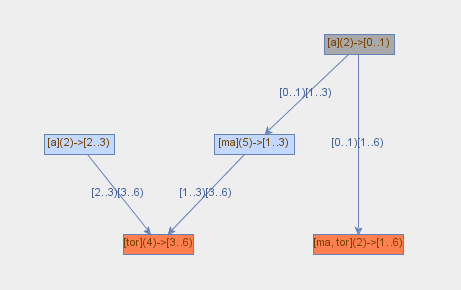
\includegraphics[width=0.7\textwidth]{figures/rosil-amator.png}
    \caption{Graful de tipare pentru cuvântul \textit{amator}}
    \label{fig:rosil-amator}
\end{figure}

\subsection{Interpretarea grafului de tipare frecvente}

Odată construit graful de tipare frecvente, se pune întrebarea dacă pe baza acestuia, se poate dezvolta o metodă de silabisire? În graful prezentat în figura \ref{fig:rosil-amator} se pot observa trei dintre cele patru tipuri de tipare (de început, de sfârsit, întermediare), stiind aceasta, se ridică întrebarea dacă caile dintre noduri de început și sfârșit reprezintă posibile despărțiri în silabe, iar dacă, care dintre acestea este despărțirea corectă?

În cazul exemplu prezentat există doua căi între noduri de început si sfârsit, acestea fiind $<a>, <ma, tor>$, respectiv $<a>, <ma>, <tor>$. Din ambele variante se ajunge la despărțirea în silabe $a-ma-tor$, care este si varianta corectă. Pornind de la această observație, în cele ce urmează vor fi prezentate o serie de strategii de selecție a căilor dintr-un graf de tipare frecvente care au probabilitate ridicată sa fie despărțiri în silabe corecte. Dar până se ajungă la aceste strategii trebuie menționat că în realitate, numărul de tipare frecvente potrivite cu un cuvânt este mult mai mare decât în exemplu demonstrativ din figura \ref{fig:rosil-amator}, iar cum căutarea tuturor căilor între două noduri este o problemă dificilă, a carei soluție depinde de complexitatea grafului analizat, este necesar o reducere a dimensiunii grafului pentru a reduce complexitatea cautării. 

\subsection{Optimizarea grafului de tipare frecvente}

Pornind de la observația de mai sus și analizând natura grafurile de tipare, se pot identifica două categorii de noduri a căror utilitate este inexistentă în vederea identificării căilor între noduri de început și noduri de sfârsit. Aceste categorii sunt:
\begin{itemize}
\item nodurile la care nu se poate ajunge din niciun nod de start.
\item nodurile din care nu se poate ajunge la niciun nod de sfârșit. 
\end{itemize}


\begin{ex}
În cadrul figurii \ref{fig:rosil-amator-prunned} se poate observa graful de tipare $G_{amator}$ după eliminarea nodurilor izolate.
\end{ex}

\begin{figure}[h!]
    \centering
    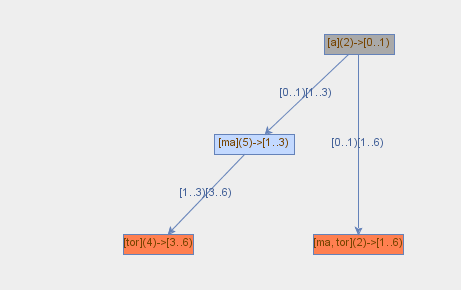
\includegraphics[width=0.6\textwidth]{figures/rosil-amator-prunned.png}
    \caption{Graful de tipare pentru cuvântul \textit{amator}}
    \label{fig:rosil-amator-prunned}
\end{figure}

Aceste noduri pot fi eliminate fără a altera soluțiile de silabisire identificate. O posibilă soluție pentru eliminarea acestora este descrisă în cadrul algoritmului \ref{algo:prunning}. 

Acesta are două etape: 
\begin{itemize}
\item O primă etapă în cadrul căreia sunt identificate nodurile care nu sunt noduri de sfârșit și nu există nicio muchie care să pornească de la acestea, respectiv nodurile care nu sunt noduri de început și pentru care nu există nicio muchie care să ajungă la ele.
\item Odată identificate aceste noduri, trebuie identificate și muchile care le au ca sursă sau destinație.
\end{itemize}
După aceste două etape, rezultă un graf posibil de dimensiune mai mică, daca acesta este cazul, cele două etape se aplică recursiv pe acesta până când în cadrul primei etape nu mai este identificat niciun nod. 

\begin{algorithm}[h!]
\SetAlgoLined
\SetKwFunction{ppg}{prunePatternGraph}

\ppg($G_{W}$) \\
\KwData{$G_{W}$ un graf de tipare descris prin $\langle V_W, E_W \rangle$}
\KwResult{$G_W'$ un graf fără noduri izolate} 

$isolatedVertices = \emptyset$ \\
\For{ $v$ \textbf{in} $V_W$}{
	\If{$deg^-(v) == 0 \wedge isNotStartNode(v)$} {
		$isolatedVertices = isolatedVertices \cup \{v\}$
	}
	\If{$deg^+(v) == 0 \wedge isNotEndNode(v)$} {
		$isolatedVertices = isolatedVertices \cup \{v\}$
	}
}

\If{$isolatedVertices == \emptyset$} {
	\KwRet $\langle V_W, E_W \rangle$
}


$edgesToBeRemoved = \emptyset$ \\
\For{ $e$ \textbf{in} $E_W$}{
	\If{$e$ \textbf{depends on a vertex from} $isolatedVertices$} {
		$edgesToBeRemoved = edgesToBeRemoved \cup \{e\}$
	}
}

$V_W' = V_W \setminus isolatedVertices$\\
$E_W' = E_W \setminus edgesToBeRemoved$\\

\KwRet \ppg($\langle V_W', E_W'  \rangle$) \\
\vspace{.1cm}

\caption{Eliminarea nodurilor izolate din cadrul unui graf de tipare}
\label{algo:prunning}
\end{algorithm}

\section{Strategii de predictie a despărțirilor în silabe}

Odată definit un graf de tipare, se pot elabora o serie de strategii prin care se stabilește care dintre căile de dintre nodurile de început și sfârșit reprezintă despărțirea corectă în silabe a cuvântului pe baza căruia a fost construit graful de tipare. 
\subsection{Identificarea căilor care pot reprezenta despărțiri în silabe}

Pentru a putea aplica strategiile menționate mai sus, este necesară identificarea tuturor căilor între nodurile de început și cele de sfârșit. Problema îdentificării tuturor câilor într-un graf este una dificilă dar în cazul grafurilor de tipare, datorită naturii lor, poate fi abordată (grafurile de tipare sunt grafuri orientate aciclice de dimensiune redusă). 

\begin{defi}
Se notează cu $I_W$ intervalul minim care conține mulțimea tuturor indexilor care pot reprezenta puncte de despărțire pentru cuvântul $W$.
\end{defi}

\begin{defi}
Fie $p_1, p_2, ..., p_n$ o cale într-un graf de tipare $G_W$, cu $p_x$ un tipar potrivit de forma $\langle tipar_x, sup_x, \left[i_x,j_x\right)\rangle$, această cale este un \textbf{lanț de tipare închis} daca 
\begin{equation}
\bigcup_{1 \leq x \leq n} \left[i_x,j_x\right) = I_W
\end{equation}
Cu alte cuvinte, un lanț de tipare închis este o cale într-un graf de tipare, pentru care primul nod este \textit{un nod de început}, iar ultimul nod este \textit{un nod de sfârșit}.
\end{defi}

Cum s-ar putea fi identificată eficient multimea tuturor lanțurilor de tipare închise? Această întrebare rămâne descrisă. Pentru a valida metoda descrisă în cadrul acestui experiment una dintre variante este ca din fiecare nod start să se realizeze explorări în lătime și reconstrucția lanțurilor de tipare închise.

\subsection{Proprietăți ale lanțurilor de tipare închise}

\begin{defi}
Fie $l$ un lanț de tipare închis dintr-o mulțime, notăm cu $s_{l}$ \textbf{silibisirea} cuvântului $W$ folosind $l$. De exemplu având lanțul de tipare închis $\langle <a>, 2, \left[ 0, 1 \right)\rangle, \langle <ma>, 5, \left[ 1, 3 \right)\rangle, \langle <tor>, 4, \left[ 3, 6 \right)\rangle$, silabisirea rezultată este $a-ma-tor$. 
\end{defi}

Ulterior se va utiliza notația $L_W$ pentru mulțimea tuturor lanțurilor de tipare închise din cadrul unui graf $G_W$.

\begin{defi}
Trebuie remarcat că există posibilitatea ca două sau mai multe lanțuri de tipare inchise pot avea aceiași silabisire asociată. Ulterior se va face referire la aceste lanțuri de tipare ca fiind \textbf{echivalente}. Fie $l_1$ și $l_2$ două tipare echivalente, în acest caz se introduce notația $l_1 \equiv l_2$.
\end{defi}

\begin{ex}
Fie $l_1 = \langle <a>, 2, \left[ 0, 1 \right)\rangle, \langle <ma, tor>, 4, \left[ 1, 6 \right)\rangle$, iar $l_2 = \langle <a>, 2, \left[ 0, 1 \right)\rangle, \langle <ma>, 5, \left[ 1, 3 \right)\rangle, \langle <tor>, 4, \left[ 3, 6 \right)\rangle$. Silabisirile asociate sunt $s_{l_1} = a-ma-tor$, respectiv $s_{l_2} = a-ma-tor$, fiind aceleași silabisiri $\Rightarrow l_1 \equiv l_2$.
\end{ex}

\begin{defi}
Considerând $l$ un lanț de tipare închis dintr-o mulțime, $L_W$, notăm cu $\vert l \vert $ \textbf{lungimea} lanțului $l$. Un lanț de lungime 2 este: $\langle <a>, 2, \left[ 0, 1 \right)\rangle, \langle <ma, tor>, 4, \left[ 1, 6 \right)\rangle$.
\end{defi}


\subsection{Strategie bazată pe numărul de căi dintre nodurile extreme}

O primă idee prin care se poate selecta lanțul de tipare închis care să reprezinte silabisirea unui cuvânt, vine de la observația de mai sus cum că din mulțimea completă de lanțuri de tipare inchise, unele sunt echivalente. 

Extinzând raționamenul, se poate pune întrebarea dacă dimensiunea claselor de echivalență poate fi folosită pentru a identifica silabisirea corectă. 

Fie $W$ un cuvânt, iar $L_W$ mulțimea tuturor lanțurilor închise identificate din graful de tipare asociat cuvântului $W$. Clasa de echivalență a unui lanț $e$ este $\left[e\right] = \{l \epsilon L_W \vert l \equiv e\}$, notându-se cu $E_{L_W}$ mulțimea tuturor claselor de echivalență a lanțurilor de tipare $L_W$. Se mai notează cu $S_{L_W}$ mulțimea tututor silabisirilor asociate cu $L_W$. Relația $f: S_{L_W} \rightarrow E_{L_W}$ este utilizată pentru a identifica clasa de echivalență asociață cu fiecare silabisire. Utilizând relația $f$, silabisirile posibile ale cuvântului $W$ pot fi ordonate în funcție de cardinalitatea claselor de echivalență. 

Prin acestă strategie se propune ca despărțirea în silabe să fie dată de cea mai numeroasă clasa de echivalentă.

\begin{ex}
.. example with graph and equivalence classes counts.
\end{ex}

\subsection{Strategie bazată pe nivelul de suprapunere}

O altă strategie pornește de la presupunerea că un nivel ridicat de suprapunere la între tiparele unui lanț închis duce la o mai bună predicție a silabisirii unui cuvânt.

\begin{defi}
Având două tipare potrivite în cadrul unui cuvânt la pentru intervalul de îndexi $[i_{P_1}, j_{P_1})$, respectiv $[i_{P_2}, j_{P_2})$ de definește nivelul de potrivire al acestor două tipare ca fiind:
\begin{equation}
\omega(P_1, P_2) = \left\{
\begin{matrix}
0, 					& j_{P_1} \leq i_{P_2}\\ 
max(i_{P_2},j_{P_1)} - min(j_{P_2},i_{P_1}),	& j_{P_1} > i_{P_2} \\
\end{matrix}
\right.
\end{equation}
\end{defi}

\begin{ex}
Pentru tiparul $P_1$ potrivit la întervalul $\left[0, 6\right)$ și tiparul $P_2$ potrivit la întervalul $\left[4, 8\right)$ avem $ \sigma(P_1,P_2)=2$
\end{ex}

\begin{defi}
Fie $l_1, l_2, ..., l_n$ un lant de tipare închis $L$. Nivelul de suprapunere pentru întreg lanțul este:
\begin{equation}
\Omega(L) = \sum_{i=1}^{n-1}{ \omega(P_i, P_{i+1})}
\end{equation}
\end{defi}

Pornind de la definiția nivelului de suprapunere de la nivelul unui lanț de tipare închis, se poate realiza o ordonare in funcție de acest nivel a lanțurilor închise din cadrul unui graf de tipare al unui cuvânt, iar ulterior să se propună ca silabisire a acelui cuvânt, silabisirea asociată cu lanțul închis cu nivel maxim de suprapunere.

\begin{ex}
.. example with graph and overlapping values.
\end{ex}

\subsection{Strategie bazată pe distanța dintre nodurile extreme}

\section{Metrici de evaluare}

\subsection{Evaluare la nivel de cuvânt}
\subsection{Evaluare la nivel de punct de despărțire}

\section{Detalii de implementare}
\subsection{Tehnologii utilizate}
\subsection{Structuri de date}
\subsection{Organizarea aplicației}
\subsection{Modularizare}